%\documentclass[a4paper,11pt,twoside,final]{book}
\documentclass[a4paper,11pt,final]{report}
%\documentclass[a4paper,11pt,final]{article}
% Pour une impression recto verso, utilisez plutôt ce documentclass :
%\documentclass[a4paper,11pt,twoside,final]{article}

\usepackage[english,francais]{babel}
\usepackage[utf8]{inputenc}
\usepackage[T1]{fontenc}
\usepackage[pdftex]{graphicx}
\usepackage{setspace}
\usepackage{array}
\usepackage[colorlinks=true]{hyperref}
\usepackage[french]{varioref}
\usepackage{listings}
\usepackage{color}
\usepackage{float}
\usepackage{wrapfig}
\usepackage{tikz}
\usepackage{comment}
\usepackage[nottoc]{tocbibind}
\usepackage{Kmelia}
\usepackage{enumitem}

\renewcommand{\lstlistingname}{Algorithme}% Listing -> Algorithm
\newcommand{\reporttitle}{Faut-il tester le modèle ou le code des composants ?}     % Titre
\newcommand{\reportauthor}{Montalvo \textsc{Araya}, Charles-Eric \textsc{Bégaudeau} et Charlène \textsc{Servantie}} % Auteur
\newcommand{\reportsubject}{X8II031\\M1 ALMA\\ 2016-2017} % Sujet
\newcommand{\HRule}{\rule{\linewidth}{0.5mm}}
\setlength{\parskip}{1ex} % Espace entre les paragraphes

\setcounter{secnumdepth}{0}

\hypersetup{
    pdftitle={\reporttitle},%
    pdfauthor={\reportauthor},%
    pdfsubject={\reportsubject},%
    pdfkeywords={rapport} {projet} {web semantique}
}

\lstset{    
            language=Kmelia,
            frame=shadowbox,
            captionpos=b,
            columns=flexible,
            breaklines=true,
            keywordstyle=\color{blue},
            stringstyle=\color{red},
            basicstyle=\ttfamily,
            numbers=left,
            numbersep=13pt,
            numberstyle=\color{gray},
            identifierstyle=\color{black},
            escapeinside={(*@}{@*)}
        }



\begin{document}
  % Inspiré de http://en.wikibooks.org/wiki/LaTeX/Title_Creation
\begin{titlepage}

\begin{center}

\begin{minipage}[t]{0.48\textwidth}
  \begin{flushleft}
    
\includegraphics [width=30mm]{images/logo-univ.png} \\[0.5cm]
    \begin{spacing}{1.5}
      \textsc{\LARGE UFR Sciences et Techniques}
    \end{spacing}
  \end{flushleft}
\end{minipage}
\textsc{\Large \reportsubject}\\[0.5cm]
\HRule \\[0.4cm]
{\huge \bfseries \reporttitle}\\[0.4cm]
\HRule \\[1.5cm]

\begin{minipage}[t]{0.4\textwidth}
  \begin{flushleft} \large
    \emph{Auteurs :}\\
    
    
    
    
    \reportauthor
  \end{flushleft}
\end{minipage}

\vfill

{\large 2017}

\end{center}

\end{titlepage}

  \cleardoublepage 
  \topskip0pt
\vspace*{\fill}
\section*{Remerciements}
\label{sec:Remerciments}


Nous aimerions remercier Pascal André, Gilles Ardourel et Jean-Marie Mottu avec lesquels nous avons travaillé au cours de ce module d'Introduction à la recherche pour leur patience et leurs explications essentielles à l'avancée de notre travail.

%L'équipe AeLos\footnote{ \url{https://ls2n.fr/equipe/AeLoS/}}
%TODO ajouter plus de remerciements ?

\vspace*{\fill}
  \tableofcontents 
  \sloppy         
  \topskip0pt
\vspace*{\fill}
\chapter*{Introduction}
\label{chap:introduction}
Ce rapport reprend le travail qui a été effectué dans le cadre du cours d'Introduction à la Recherche du master 1 ALMA 2017 par notre groupe composé de Montalvo Araya, Charles-Eric Begaudeau et Charlène Servantie.


Le sujet sur lequel nous avons travaillé est : "Faut-il tester le modèle ou le code des composants ?", un sujet proposé par Pascal André, Jean-Marie Mottu et Gilles Ardourel de l'équipe AeLoS\footnote{Architectures et Logiciels Sûrs, \url{https://ls2n.fr/equipe/AeLoS/}}, qui ont été nos encadrants au cours de cette découverte du monde de la recherche.

Nous avons tout d'abord choisi de présenter le modèle Kmelia, le framework COSTO et les concepts abordés dans le chapitre~\ref{chap:KmeliaCOSTO}, à travers notamment les différents articles que nous avons été amenés à lire pour appréhender le sujet de recherche. Ensuite nous allons parler dans le chapitre~\ref{chap:harnais} sur le test de modèle à travers le générateur de harnais de COSTOTest, puis nous présenterons l'utilisation de JUnit pour faire du test sur le code Java généré et notre processus de travail pour générer ces tests dans le chapitre~\ref{chap:JUnit}. Nous avons ensuite comparé le test de modèle avec le test de code dans le chapitre~\ref{chap:comparaison}, où nous discutons également de notre travail et de nos blocages au cours de ce travail. Enfin, nous avons essayé d'apporter des réflexions sur de nouveaux tests et l'analyse de mutation au chapitre~\ref{chap:mutations}

%alias la partie 4, bref, lien vers la partie
  %plan
  %modèle kmelia
  %générateur de harnais de test pour le model testing
  %test java JUnit focus sur processus + méthodologie
  %comparaison model testing/ testing junit
  %mutations / autre exemple, autre service
 

\vspace*{\fill}
  \clearpage
  %modèle kmelia
  \chapter{Kmelia et le framework COSTO}
\label{chap:KmeliaCOSTO}
\begin{comment}
    
    The main features of Kmelia are:
    
    component : a component is a container of services; it is described with a state space constrained by an invariant. A component is designed independently from its environment by setting assumptions such as virtual client components or required service specifications;
    
    service: a service describes a functionality; it is more than a simple operation; it has a pre-condition, a post-condition and a behaviour described with a labelled transition system (LTS). Moreover a service may hierarchically give access to other services. The behaviour supports communication interactions, dynamic evolution rules and service composition;
    
    assembly of components: an assembly is a set of components linked via their required and provided services with the aim to build effective functionality. Linking components by their services in assemblies establishes a possible bridge to Service Oriented Architectures. The component assemblies are governed by strict service composability rules;
    
    composite component: a composite component is a component that encapsulates assemblies or other components; it is subject to encapsulation and promotion policies.
\end{comment}


\section{Contexte}
\label{sec:contexte}
    Pour ce travail de recherche, nous avons été amenés à utiliser le framework COSTO ainsi que le langage de modélisation Kmelia, que nous présentons dans cette partie.

    Nous avons choisi de reprendre certains des concepts sur lesquels reposent les travaux que nous avons lu pour pouvoir avoir une trace de l'ensemble des concepts avec lesquels nous avons été amenés à travailler au cours de ce travail et permettre une meilleure compréhension de l'ensemble.
    

\subsection*{L’équipe AeLos}
    L'équipe AeLos\footnote{Architectures et Logiciels Sûrs \url{https://ls2n.fr/equipe/AeLoS/}} est une équipe du LS2N\footnote{Laboratoire des Sciences du Numérique de Nantes par lesquels ils sont définis. \url{https://ls2n.fr/}} dirigée par Christian Attiogbé. AeLos travaille sur plusieurs axes de recherche en lien avec le développement de logiciels sûrs et les modèles. 
\clearpage

\section{Notions de test}
\label{sec:notionTest}

    Comme l'explique P. André et al. dans \cite{amaretto17} dans le développement dirigé par les modèles, il est important de vérifier que le modèle abstrait est correct pour avoir un résultat le plus sûr possible.   
    Cette vérification demande une combinaison de techniques de tests car on a un système comprenant des composants basés sur des services requis et des services fournis. Ce système a trois types de propriétés chacune vérifiée par une méthode spécifique : 
    \begin{itemize}[label=\textbullet, font=\large]
        \item interaction, vérifiée par model checking, 
        \item cohérence, vérifiée par theorem proving, 
        \item conformation du comportement au contrat fonctionnel, vérifiée par model testing spécifique.
    \end{itemize}

\subsection*{Développement dirigé par les modèles}
    Le développement dirigé par les modèles (souvent abrégé en MDD, pour Model-driven Development) est un type de développement basé sur une représentation du problème posé avec des méta-modèles et des modèles qui permettent également de décrire la solution que l'on souhaite apporter à ce problème.
    On utilise souvent un langage de modélisation  pour représenter le problème ainsi que les solutions qu'on y apporte, et un exemple connu est l'UML\footnote{Unified Modeling Language, est un langage de modélisation graphique, permettant la création de diagramme représentant le logiciel ou programme, \url{http://www.uml.org}}. Le langage Kmelia en est un autre exemple, sur lequel nous en parlerons plus en détails dans la section~\ref{sec:KmeliaCOSTOLangage}.
    
\subsection*{Vérification et Validation}
    
    Dans le cadre du développement de produit, et notamment de produit informatique, on teste la qualité du produit en utilisant à la fois de la vérification et de la validation.
    
    La vérification correspond au test de correction d'une phase ou de l'ensemble. On vérifie que le produit fait ce qui est demandé sans bugs ou erreurs de réalisation.
    
    La validation quant à elle repose sur la conformité du produit avec ce qui a été demandé par le client, c'est à dire que la réalisation convient aux spécifications et répond aux besoins exprimés.
    
\subsection*{Model Checking}

    La vérification de modèles, ou model checking, consiste à tester si les propriétés d'interaction d'un modèle sont satisfaites. 
   

\subsection*{Model Testing}

    Le test de modèles, ou model testing, consiste à réaliser des tests en boite noire en ce basant sur un modèle abstrait. On vérifie que le code correspond bien au modèle. Le harnais de test que nous aborderons dans la section~\ref{chap:harnais} fonctionne sur ce principe.
    
    La démonstration par expérimentation a été faite avec le langage de description de modèle Kmelia et l'outil COSTO, et l'article précise qu'il faut plus de travail et d'amélioration des outils pour avancer, notamment sur la partie de la spécification et de la vérification de la qualité de service. Il faut également de nouveaux éléments de langage pour les contraintes de temps et de ressources, ce qui nécessite des tests des techniques de vérification et validation associées.

\subsection*{Platform Independent Model PIM}
    
    C'est le modèle logiciel qui est indépendant de l'implémentation du logiciel (langage, \dots ). Ce terme est fréquemment utiliser dans le contexte d'une approche de l'architecture du logiciel basé sur les modèles. L'idée est de baser l'architecture du logiciel sur son modèle pour la rendre indépendante d'une quelconque plateforme d'implémentation. 
    
    Il existe des outils  spécialisés pour ce genre d'approche tels que VIATRA, ATLAS  ou Kmelia (CostoTest).

\subsection*{Component Testing}
    
    Ce type de test est utilisé dans les logiciels à composants. Pour s'assurer de la correction du logiciel il est nécessaire de s'assurer de la fiabilité de chacun de ses composants de manière individuelle. 
    
    Ce genre de test se concentre sur un composant à la fois ce qui nécessite dans la plus part des cas de créer des mocks pour simuler les autres composants que le composant sous test requiert pour fonctionner.

\section{Langage Kmelia}
\label{sec:KmeliaCOSTOLangage}

\begin{comment}
    language to describe a component model based on the description of complex services. Kmelia components are abstract, independent from their environment and therefore non-executable.
    Kmelia can be used to model software architectures and their properties, these models being later refined to execution platforms. It can also be used as a common model for studying component or service model properties (abstraction, interoperability, composability). Kmelia main characteristics are: components, services, software architectures, protocols, contracts, specification of complex interaction between services.
    
    Kmelia est un langage à composants multi-services. On distingue les services offerts qui réalisent des fonctionnalités et les services requis qui déclarent les besoins du composant. Ce langage permet de modéliser des composants logiciels, des architectures logicielles par assemblage avec leurs propriétés, afin de permettre une bonne lisibilité, flexibilité et une bonne traçabilité dans la conception des architectures. Kmelia répond aux besoins suivants :
    Une réelle réutilisation des composants.
    Un modèle indépendant des plateformes d’exécution.
    Un langage de spécification de composants, de services et de leur assemblage.
    Un cadre de développement de composants afin d’élaborer des composants corrects par construction et raisonner sur des assemblages des composants.
    Les analyses de propriétés des spécifications Kmelia sont mises en œuvre dans la plateforme d’expérimentation ouverte Costo, sous forme d’un ensemble de plugins Eclipse.


\end{comment}

    Le langage Kmelia\cite{Kmelia} est un langage de modélisation développé par l'équipe AeLoS, qui permet de décrire des modèles de composants basés sur des services eux-mêmes décrits par Kmelia. Les composants ainsi créés par Kmelia sont indépendant de l'environnement d'exécution et donc non exécutables, ce qui permet de s'affranchir de la contrainte de la plate-forme sur laquelle le programme sera exécuté. 

    Ce langage permet de spécifier les services requis par un composant ainsi que ceux qu'il fournit. Ceci permet de modéliser des systèmes complexes en garantissant autant que possible une bonne lisibilité de la conception et une  indépendance de la plateforme d'exécution, ce qui permet également d'avoir des composants réutilisables et de faire de l'assemblage de composants.

    La génération de code et l'analyse de ses spécifications ont été mises en oeuvre dans la plateforme COSTO, sous forme de plugins Eclipse.

\begin{lstlisting}[frame=single, caption={Exemple de fichier Kmelia décrivant un composant},label=fig:KmeliaVehicleTester]
COMPONENT VehicleTester
INTERFACE  
  provides : {testcase1}
  requires : {computeSpeed} 
  autorun: {testcase1}
USES {PLATOONTESTLIB,PLATOONLIB,DEFAULT} 
VARIABLES    
  obs verdict: Boolean ;
SERVICES

provided testcase1 ()
Interface
  extrequires: {computeSpeed}   
Variables
computespeedresult : Integer;
Sequence
{   
 # init sequence
 # call
  computespeedresult:= (*@ \text{!!} @*)computeSpeed(getData("safeDistance"));
  # oracle evaluation
  verdict:= (computespeedresult = getData("oracledata"));
  # transmit verdict
  assertT(verdict);
  #end of service
  SendResult()
  }
End

required computeSpeed(safeDistance : Integer) : Integer
End
END_SERVICES

\end{lstlisting}

On peut constater que le .kcp contient :
\begin{itemize}[label=\textbullet, font=\large]
    \item {\scshape component} qui définit le nom du composant,
    \item {\scshape interface} qui liste les compinterface, les interfaces du composant,
    \item {\scshape uses} qui liste les complibclause utilisés par le composant,
    \item {\scshape variables} qui liste les compobservvariablesclause, les variables observables du composant,
    \item {\scshape services} description des services du composant et de leur fonctionnement,
    \item provided qui liste les services fournis par le composant,
    \item Interface  qui liste les servinterface, les interfaces du services,
    \item Variables qui liste les servvariablesclause, les variables du services
    \item required qui liste les services nécessaires au fonctionnement du composant,
\end{itemize}

\clearpage
\section{Framework COSTO}
\label{chap:KmeliaOutilDeTestCOSTO}
    COSTO est un outil qui se présente sous la forme de plugins pour Eclipse permettant notamment de générer du code à partir de fichiers Kmelia.

    Cet ensemble de plugins a été développé pour supporter la spécification et l'analyse des systèmes de composants Kmelia. Il gère les spécifications Kmelia et la vérification des propriétés primaires (analyse syntaxique, vérification de type, analyse statique,...)\cite{rapportM2}.

    COSTO utilise notamment le framework ANTLR\footnote{\url{http://www.antlr.org/about.html}} pour la reconnaissance du langage Kmelia et son interprétation. ANTLR prend en entrée une grammaire formelle définissant un langage et produit le code reconnaissant ce langage.

    Le framework fournit une interface \textit{IService} pour la gestion des services. Pour pouvoir appelé les services le framework fournis aussi des \textit{IChannel}. Les channels appellent et récupère les données renvoyées pour un service donnée. 

    Un composant utilisant le framework a des \textit{IProvidedService} qui sont les services fournis par le composant. Un composant possède aussi des \textit{IRequiredService} qui sont les services nécessaire pour le fonctionnement du composant.

    Il dispose également d'un plugin COSTOTest qui permet de générer des harnais de tests à partir du code qui a été généré par COSTO depuis des fichiers Kmelia. Le plugin permet de faire des tests sur des services précis et peut créer des mocks qu'on lui demande tout seul. 

\clearpage
\subsection*{Les channels}
\label{subsec:channels}
    Le langage Kmelia est un langage qui utilise des \textit{goto}s, ce que le langage Java ne permet pas, à cause de cela le code généré doit imité cette fonctionnalité du langage de modélisation et donc crée des classes \textit{{\bfseries nom-classe}LTS} comme : 
    \begin{itemize}[label=\textbullet, font=\large]
        \item SimpleDriver\_{}giveSafeDistance
        \item SimpleDriver\_{}giveSafeDistanceLTS
    \end{itemize}
    La première contenant la second et l'initialisant comme ceci :
    
\lstset{    
            language=Java,
            frame=shadowbox,
            captionpos=b,
            columns=flexible,
            breaklines=true,
            keywordstyle=\color{blue},
            stringstyle=\color{red},
            basicstyle=\ttfamily,
            numbers=left,
            numbersep=13pt,
            numberstyle=\color{gray},
            identifierstyle=\color{black},
            escapeinside={(*@}{@*)}
        }

\begin{lstlisting}[frame=single, caption={Initialisation d'un LTS},label=fig:initLTS]
    public void initLTS(){
        (*@ \text{{\bfseries nom-classe}LTS} @*) lts =
            new (*@ \text{{\bfseries nom-classe}LTS} @*)();
        this.setLTS(lts);
        lts.setService(this);
        lts.init();
    }
\end{lstlisting}

\subsection*{La fonction callService()}
    %		serv.callService("_goalreached", "goalreached",new Object[]{mylib.PlatoonTestlibMap.getData("safeDistance")}, serv);

CallService est une fonction de l'interface IService qui appelle un Service en prenant les paramètres suivant : 
    \begin{itemize}[label=\textbullet, font=\large]
        \item le nom du channel, il est normalement sous la forme \_{}{\bfseries nom-du-service}
        \item le nom du service,
        \item les paramètres d'on le service a besoin. Attention ceux-ci ne sont pas les services requis,
        \item le service sur le quel on appelle la fonction ,
    \end{itemize}
Vous pourrez retrouver en annexe le diagramme de séquence de la fonction callService~\ref{annexe:callServiceSeq} et de callService avec le mock testChannel~\ref{annexe:callServiceSeqMock}.

\begin{lstlisting}[frame=single, caption={Initialisation d'un LTS},label=fig:initLTS]
IProvidedService serv = driv.getProvidedService("pos");
	
serv.callService("_pos", "pos",
  new Object[]{mylib.PlatoonTestlibMap.getData("safeDistance")},
  serv);
\end{lstlisting}
  %\clearpage
  %générateur de harnais de test pour le model testing
  %\chapter{Génération des harnais de tests, Model testing}
\chapter{Test du modèle et génération du harnais}
\label{chap:harnais}

Ce chapitre est basé principalement sur les recherches précédentes des étudiants de Master 1 et de Master 2 dont nous avons utilisé les rapports pour avancer dans notre travail.

Notre objectif étant d'effectuer une comparaison entre le test du modèle et le test du code, comme le travail sur le test du code avait déjà été effectué en amont par le groupe d'étudiants de Master 2\cite{rapportM2}, nous nous sommes documentés sur cette étape sans y apporter de nouvelles informations. 

Ce chapitre repose principalement sur les rapports des étudiants précédents et sur la documentation disponible sur le site de COSTO\footnote{\url{http://costo.univ-nantes.fr/}}. Nous avons choisi de reprendre ces informations parce que nous avons passé du temps à les comprendre et qu'il nous parait important d'avoir une explication du modèle et de la génération du harnais au sein de ce rapport.



\section{Modèle utilisé : Platoon System}
\label{sec:harnaisModele}

Pour le test du modèle et la génération du harnais, nous avons travaillé avec l'exemple du PlatoonSystem\footnote{\url{http://costo.univ-nantes.fr/application/vehicle-exemple/}} qui est un modèle représentant un système de véhicules qui se suivent avec un pilote au départ. Ce modèle est représenté schématiquement par la figure \ref{fig:platoonSchema} avec les services fournis et requis. Ces véhicules doivent répondre à des contraintes de vitesse minimale, maximale et de distance de sécurité, chaque véhicule modifiant sa vitesse en fonction de celle du véhicule devant lui.

\begin{figure}[H]
    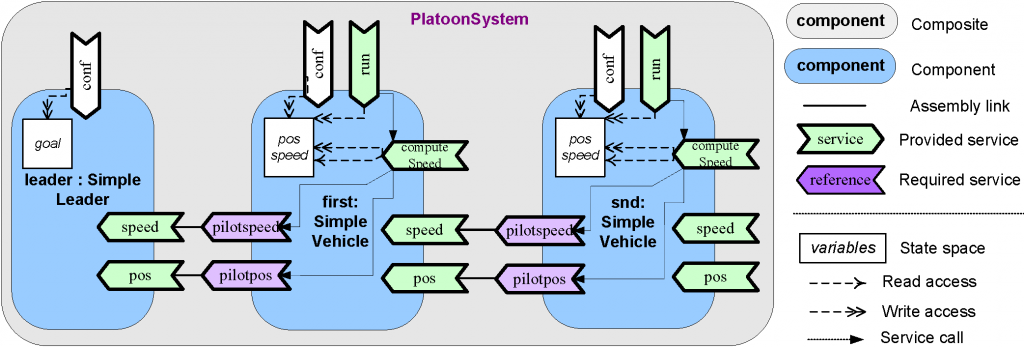
\includegraphics[scale=0.35]{images/platoonSchema.png}
    \caption{Schéma du PlatoonSystem}
    \label{fig:platoonSchema}
\end{figure}


\section{Génération du harnais de test}
\label{sec:harnaisGeneration}

COSTOTest est le plugin servant à générer et lancer les harnais de tests, on l'utilise en lançant Eclipse avec la bonne installation\footnote{\url{http://costo.univ-nantes.fr/tools/technical-environment-of-costo/eclipse-installation/}}

Pour lancer le harnais il faut cliquer sur \textit{GenerateTH}, ensuite il faut sélectionner le service à tester. Ensuite le plugin affiche une fenêtre où il est possible de placer des mocks sur les services nécessaires au test. Une fois que tout est paramétré, il est possible de lancer le harnais de test. Une fenêtre s'ouvre et permet de choisir quelle valeur les mocks doivent renvoyer, le harnais procède à un test sur ces valeurs et génère un fichier de verdict. Par la suite il est possible de réutiliser un harnais de test sans devoir le re-paramétrer si on souhaite faire un test sur des valeurs. Il est aussi possible de tester plusieurs jeux de valeurs en même temps il suffit de préciser le nombre que l'on souhaite et de fournir les données de tests.
\clearpage
    \topskip0pt
    \vspace*{\fill}
\begin{figure}[H]
    \begin{center}
        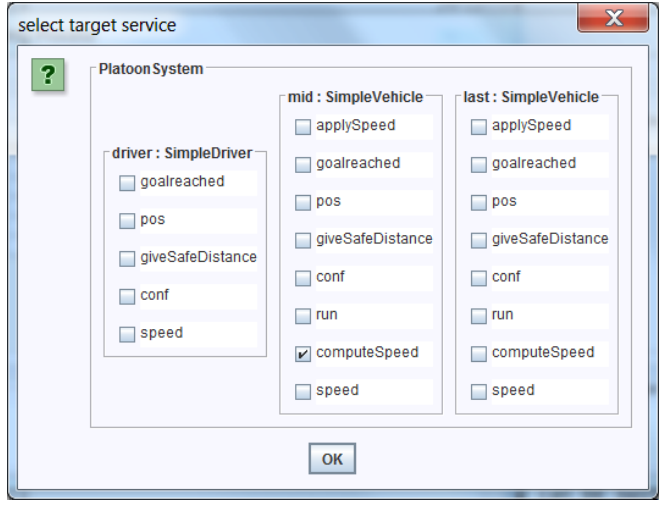
\includegraphics[scale=0.8]{images/SelectionServiceCOSTOTest.png}
        \caption{Image sélection de service COSTOTest}
        \label{fig:SelectionServiceCOSTOTest}
    \end{center}
\end{figure}

    \vspace*{\fill}
    \clearpage
    \topskip0pt
    \vspace*{\fill}
 
 Voici l'écran sur lequel on peut rentrer les valeurs de test et où on peut créer des mocks. 
\begin{figure}[H]
    \begin{center}
        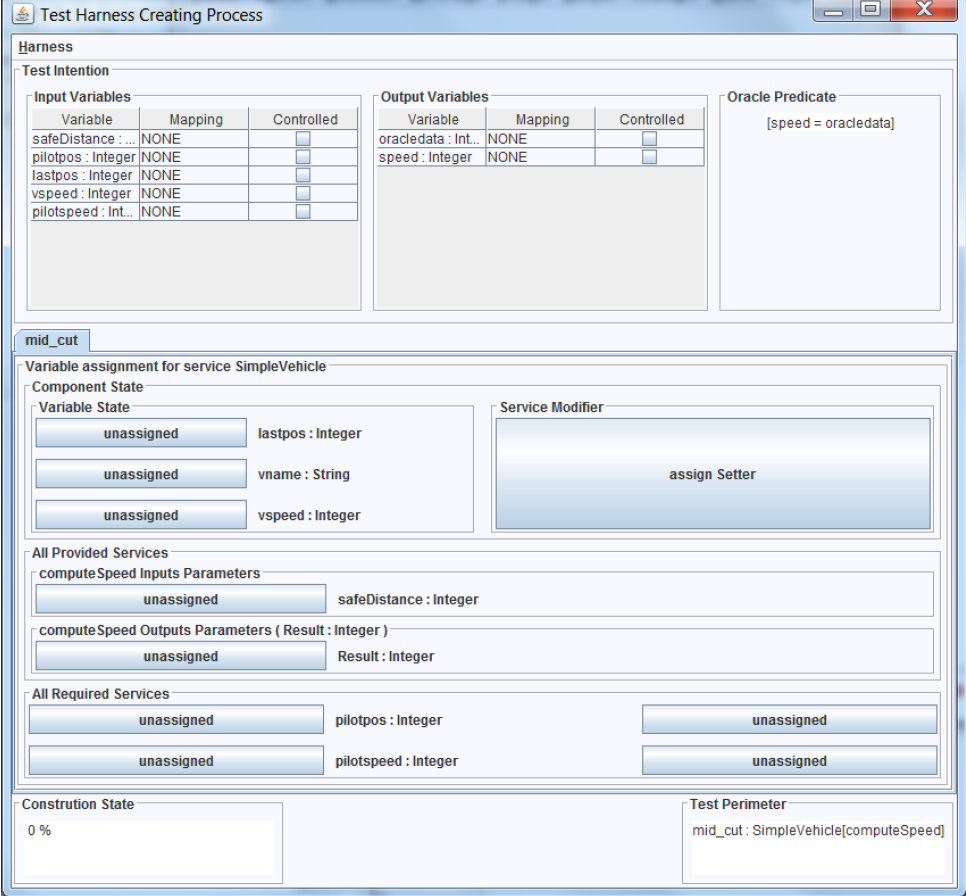
\includegraphics[scale=0.6]{images/CreationMockCOSTOTest.png}
        \caption{Image sélection des valeur du test et crétion des mocks COSTOTest}
        \label{fig:CreationMockCOSTOTest}
    \end{center}
\end{figure}

    \vspace*{\fill}
    \clearpage
    \topskip0pt
    \vspace*{\fill}

Et voici à quoi ressemble un harnais de test complété sur le service \textit{computeSpeed}
\begin{figure}[H]
    \begin{center}
        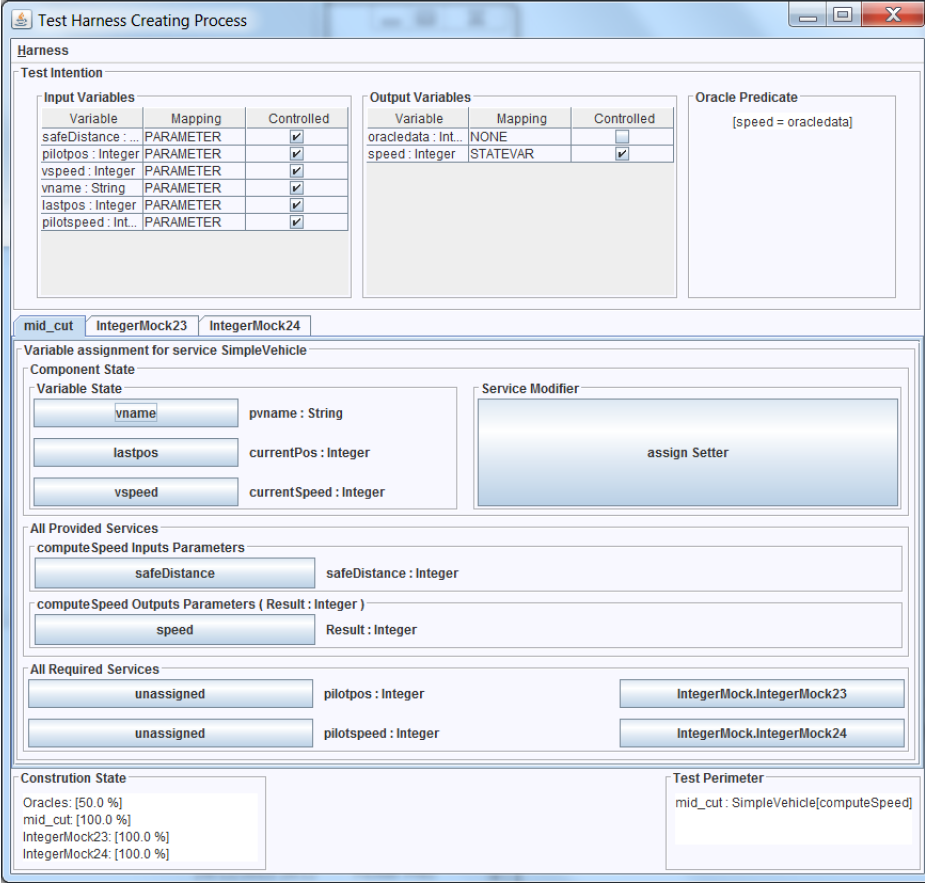
\includegraphics[scale=0.55]{images/HarnaisFiniCOSTOTest.png}
        \caption{Harnais complété COSTOTest}
        \label{fig:SelectionServiceCOSTOTest}
    \end{center}
\end{figure}

    \vspace*{\fill}


  %\clearpage
  %test java JUnit focus sur processus + méthodologie
  \chapter{Test du code Java avec JUnit}
\label{chap:JUnit}

\section{Mise en place}
\label{sec:JUnitMiseEnPlace}
Pour notre travail, nous avons utilisé la version standalone contenant les plugins COSTO et Eclipse, mais également effectué l'installation des différents plugins sur Eclipse Juno car une partie d'entre nous utilisait une distribution Linux. 

Pour pouvoir garder les différentes versions de notre travail ainsi que pour pouvoir mieux travailler en groupe nous avons utilisé un dépôt Git\footnote{\url{https://github.com/E1drad/COSTO}}.

Nous avons travaillé avec la version 4 de la librairie JUnit\footnote{\url{http://junit.org/junit4/}}, et nous avions commencé à travailler avec Mockito\footnote{\url{http://site.mockito.org/}} avant d'en abandonner l'usage car cela nous posait des soucis de version de JRE  et qu'il était plus intéressant et potentiellement plus simple de chercher à faire nos mocks par nous-même.

Notre objectif étant d'établir un test du code généré, nous avons donc créé un nouveau package\footnote{kmelia.autonomousSimplePlatoon.testsM1IR} dans lequel créer nos tests, de manière à ce qu'ils ne disparaissent pas si jamais nous régénérions le test pour une raison ou une autre.

\clearpage
\section{Processus}
\label{sec:JUnitProcessus}

Nous nous sommes renseignés sur les pratiques de tests unitaires ainsi que les séries de tests notamment grâce à l'ouvrage Tests Unitaires en Java \cite{testUnit} conseillé par nos enseignants référents.

Pour faire du test unitaire, il faut isoler le composant à tester du système et notamment de ses services requis de manière à pouvoir réellement tester le composant uniquement, et pas toute l'architecture sur laquelle il s'appuie derrière.

Ceci implique de prévoir des mocks pour simuler ces services et n'étudier que le comportement du composant. 

Nous avons commencé dans notre travail par chercher à comprendre les différents appels de services effectués par le système dans l'exemple du PlatoonSystem.\footnote{Dont la mise en place est expliquée ici :\\ \url{http://costo.univ-nantes.fr/application/vehicle-exemple/}}


Au tout début nous avions voulu tester le service \textit{computeSpeed} de la classe \textit{SimpleVehicle} mais comme ce service était plutôt compliqué car il nécessite d'autres services pour fonctionner nous avons d'abord testé des services plus simple comme le service \textit{pos} et \textit{goalreached}.



Cela nous a permis de nous familiariser avec le système des channels du framework. Cependant nous nous sommes vite rendus compte qu'il serait plus simple d'utiliser des mocks pour les channels et nous avons donc créé une classe \textit{TestChannel} qui est un mock qui simule le fonctionnement d'un channel.


Nous avons travaillé à la génération de test pour la méthode computeSpeed(). Nous avons utilisé la classe \textit{TestChannel} pour ces tests. Pour les tests sur \textit{computeSpeed} d'un \textit{SimpleVehicle} nous avons assigné un \textit{TestChannel} au service \textit{computeSpeed} du véhicule. ComputeSpeed étant un service nécessitant les services pilotpos et pilotspeed nous avons créé des mocks sur ces services en utilisant \textit{TestChannel}, ce channel fournit aussi une \textit{safeDistance} car computeSpeed en a également besoin. Ensuite il suffit de fournir les valeurs que nous voulons via les mocks puis de récupérer le résultat de computeSpeed() pour faire les tests. 


\section{Blocages}
\label{sec:JUnitBlocages}

L'ensemble de l'architecture du système nous a posé quelques soucis de compréhension lors de nos travaux. 

Nous avons notamment bloqué pendant une longue période sur la compréhension du langage Kmelia, du fonctionnement de COSTO et de la génération du harnais de test par COSTOTest, même si nous n'avions pas besoin d'une compréhension en profondeur de tout le système.

Nous avons également tenté une approche réflexive sur laquelle nous avons rapidement bloqué à cause des channels (voir \ref{subsec:channels})

\begin{lstlisting}[frame=single, caption={exemple de fonction généré},label=fig:isGuardSatisfied]
public Boolean isGuardSatisfied(String transition) {
    if (transition==null) 
        return false;
    if ("i___i1___1".equals(transition)) 
        return this.service.guard_i___i1___1();
    if ("i1___f___2".equals(transition)) 
        return this.service.guard_i1___f___2();
    return true;
}
\end{lstlisting}


\subsection*{Channel}
    Nous avons eu du mal à comprendre à comment se servir des channels pour appeler les services et recevoir leurs résultats. Notamment comprendre comment fonctionne la fonction \textit{callService()}  qui est la fonction qui permet d'appeler les services via un channel.
    
    Par la suite nous avons utilisé une classe qui est un mock de la classe Channel pour pouvoir faire les tests plus facilement.

\clearpage

\section{Code}

\lstset{    
            language=Java,
            frame=shadowbox,
            captionpos=b,
            columns=flexible,
            breaklines=true,
            keywordstyle=\color{blue},
            stringstyle=\color{red},
            basicstyle=\ttfamily,
            numbers=left,
            numbersep=13pt,
            numberstyle=\color{gray},
            identifierstyle=\color{black},
            escapeinside={(*@}{@*)}
        }


Voici le code de la classe TestChannel que nous a fourni M. Ardourel pour pouvoir faire un mock de channel pour utiliser dans nos tests.
\begin{lstlisting}[frame=single, caption={TestChannel.java},label=fig:JUnitTestChannel]
package kmelia.autonomousSimplePlatoon.testsM1IR;
/**
 * Classe mock channel fournie par Gilles Ardourel
 */
public class TestChannel extends Channel{
    private Object result;
    private Object[] callparams;
    private Map<String,Object[]> mockvalues;
    public void setCallparams(Object... callparams) {
    	this.callparams = callparams;
    }   
    /**
     * @param callname name of the required service to mock
     * @param values results to be returned by the
     * mocked service
     */
    public void addMockValue(String callname, Object...values){
    	mockvalues.put(callname, values);
    }    
    public Object getResult() {
    	return result;
    }    
    public TestChannel(String name, IService client,
        IService server) {
    	super(name, client, server);
    	mockvalues= new HashMap<>();
    }    
    public void clearMockValue(){
    	mockvalues.clear();
    }    
    @Override
    public Object[] receiveMessage(String channel, 
        String message, Class<?>[] paramtypes,
        IService orig) {
    	System.err.println(" the Service wants to "
    	    + "receive a message, use a mock "+message);
    	return null;
    }    
    @Override
    public void emitMessage(String channel, String message, 
        Object[] params, IService orig) {
    	System.out.println(" the Service emits "+message);
    }    
    @Override
    public void callService(String channel, String message, 
        Object[] params, IService orig)
        throws KmlCommunicationException {
    	System.out.println("the service calls another "
    	    + "Service "+channel+" "+message);
    }    
    @Override
    public void returnService(String channel, String message, 
        Object[] params, IService orig) {
    	System.out.println("the service "+message+" returns "+
    	    params[0]);
    	orig.ack(this,0);
    	result=params[0]; 
    }    
    @Override
    public Object[] receiveServiceCall(String channel, 
        String message, Class<?>[] paramtypes, IService orig) {
    	return this.callparams;
    }    
    @Override
    public Object[] receiveServiceReturn(String channel, 
        String message, Class<?>[] paramtypes, IService orig) {
    	
        return mockvalues.get(message);
    }    
    @Override
    public void close(IService source) {
    	// Overriding to NOP because this channel is one-ended
    }    
    @Override
    public void cut(IService source) {
    	// Overriding to NOP because this channel is one-ended
    }
}
\end{lstlisting}

\clearpage

A partir de ce TestChannel, cela nous a permis de créer une suite de tests pour tester la méthode computeSpeed(). Pour faciliter la lecture des test à partir du deuxième test, nous avons supprimé les parties qui ne changent pas, le code complet étant disponible sur notre dépôt git. 
Voici le code :

\begin{lstlisting}[frame=single, caption={TestOnComputeSpeed.java},label=fig:JUnitTestOnComputeSpeed]
package kmelia.autonomousSimplePlatoon.testsM1IR;

public class TestOnComputeSpeed {
    /**
     * Test quand le vehicle est suffisament loin du driver.
     * @throws InterruptedException
     * @throws KmlCommunicationException
     * @throws ServiceException
     */
    @Test
    public void testComputeSpeedOk() 
        throws InterruptedException,
        KmlCommunicationException, ServiceException{		

        SimpleVehicle veh = new SimpleVehicle("SimpleVehicle", 
        new TestOuterContext("test"),"last");
        int posValue=10;
        veh.setConfig("conf","last",posValue,0);
        veh.init();	
        
        IProvidedService provServToTest =
            veh.getProvidedService("computeSpeed");
            
        //Create and assign fake test channel 
        TestChannel testChan = new TestChannel(
            "TESTCHANN",null,provServToTest);
        provServToTest.assignChannel(testChan);
        veh.getRequiredService("pilotpos")
            .setReqChannel(testChan);
        veh.getRequiredService("pilotspeed")
            .setReqChannel(testChan);		
            
        //assigning call parameters for Service under test
        testChan.setCallparams(120);// safeDistance
        testChan.addMockValue("pilotpos", 420);
        testChan.addMockValue("pilotspeed", 40);	
        
        provServToTest.start();
        
        Thread.sleep(1000); 
        
        provServToTest.stop(testChan);
        
        System.out.println(testChan.getResult());
        assertEquals(true,
            (Integer)testChan.getResult()>0);	
    }	
	
    /**
     * Test quand le vehicle est trop proche du driver
     * @throws InterruptedException
     * @throws KmlCommunicationException
     * @throws ServiceException
     */
    @Test
    public void testComputeSpeedTropProche() 
        throws InterruptedException, 
        KmlCommunicationException, ServiceException{	
            [...]
        int posValue=10;	
            [...]
        testChan.setCallparams(120); // safeDistance
        testChan.addMockValue("pilotpos", 40);
        testChan.addMockValue("pilotspeed", 40);	
            [...]
        System.out.println(testChan.getResult());
        assertEquals(true,
            (Integer)testChan.getResult()==0);
    }	
    /**
     * Test quand le vehicle est devant le driver
     * @throws InterruptedException
     * @throws KmlCommunicationException
     * @throws ServiceException
     */
    @Test
    public void testComputeSpeedDevantDriver() 
        throws InterruptedException, 
        KmlCommunicationException, ServiceException{	
            [...]
        int posValue=100;	
            [...]
        System.out.println(testChan.getResult());
        assertEquals(true,
            (Integer)testChan.getResult()==0);
    }	
    /**
     * Test quand le driver va tres vite.
     * Cela ne doit normalement pas affecter le vehicule
     * @throws InterruptedException
     * @throws KmlCommunicationException
     * @throws ServiceException
     */
    @Test
    public void testComputeSpeedDriverRapide()
        throws InterruptedException, 
        KmlCommunicationException, ServiceException{	
            [...]
        int posValue=10;
        veh.setConfig("conf","last",posValue,0);
        veh.init();	
            [...]
        System.out.println(testChan.getResult());
        assertEquals(true,(Integer)testChan.getResult()>0);
    }	
    /**
     * Test quand la safe distance est negative
     * @throws InterruptedException
     * @throws KmlCommunicationException
     * @throws ServiceException
     */
    @Test
    public void testComputeSpeedNegativeSafeDistance() 
        throws InterruptedException, 
        KmlCommunicationException, ServiceException{	
            [...]
        int posValue=10;		
        veh.setConfig("conf","last",posValue,20);
        veh.init();	
            [...]
        testChan.setCallparams(120); //safeDistance
        testChan.addMockValue("pilotpos", 400);
        testChan.addMockValue("pilotspeed", 4000);	
            [...]
        System.out.println(testChan.getResult());
        assertEquals(true,(Integer)testChan.getResult()>0);	
	}	
    /**
     * Test quand le vehicule a deja une vitesse
     * @throws InterruptedException
     * @throws KmlCommunicationException
     * @throws ServiceException
     */
    @Test
    public void testComputeSpeedDejaLancer() 
        throws InterruptedException, 
        KmlCommunicationException, ServiceException{	
            [...]
        int posValue=10;		
        veh.setConfig("conf","last",posValue,20);
        veh.init();		
            [...]
        //assigning call parameters for Service under test
        testChan.setCallparams(-1); //safeDistance
        testChan.addMockValue("pilotpos", 400);
        testChan.addMockValue("pilotspeed", 4000);	
            [...]
        System.out.println(testChan.getResult());
        assertEquals(true,(Integer)testChan.getResult()>0);
    }
}

\end{lstlisting}
  %\clearpage
  %comparaison model testing/ testing junit
  \chapter{Comparaison entre le harnais de test et JUnit}
\label{chap:comparaison}

    \begin{figure}[H]
        \begin{center}
          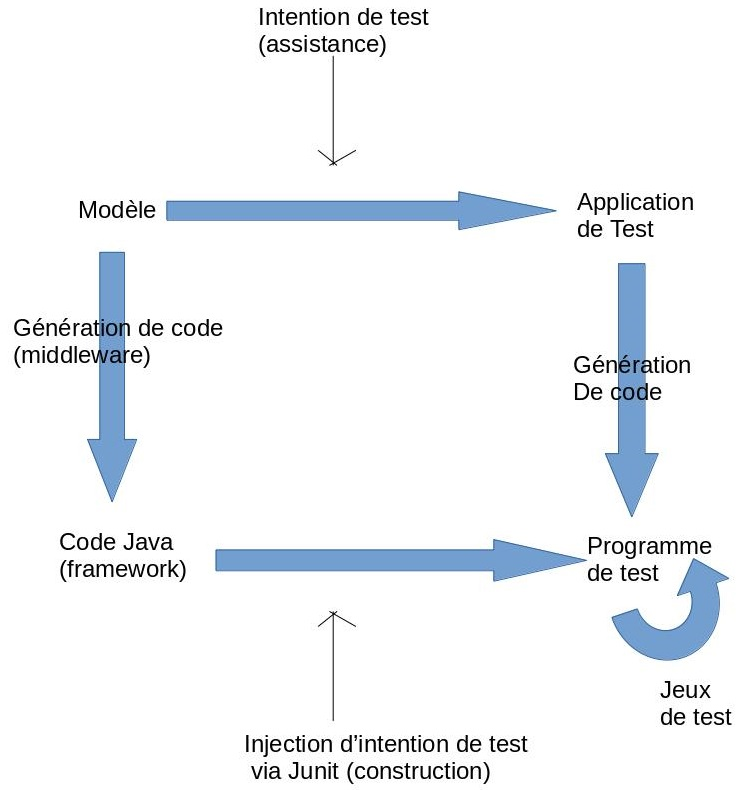
\includegraphics[scale=0.5]{images/structSchema.jpg}
          \label{fig:StructModelTests}
          \caption{Structure des tests sur le modèle par assistance ou construction}
        \end{center}
    \end{figure} 

Sur la figure ci-dessus, on peut voir les deux manières de tester un modèle, soit à la manière du harnais de tests créés par COSTOTest en utilisant les intentions de tests Kmelia, soit comme nous avons cherché à le faire en générant du code conforme au modèle que nous testons ensuite manuellement en injectant nos intentions de tests via JUnit.

L'hypothèse de départ est qu'il est plus rentable en terme de temps de générer les tests sur le modèle et non pas sur le code généré à partir du modèle.

\section{Intérêts du test sur le modèle par rapport à Junit}

Grâce à l'utilisation du générateur de harnais de tests dans COSTOTest en suivant la procédure indiquée dans la documentation, la génération du test de computeSpeed() est relativement rapide à mettre en place, les fonctionnalités du plugin permettant d'intégrer les données multiples en une seule fois grâce à un fichier .csv contenant les données d'entrée et les oracles pour les tests.

De plus, la présence et l'utilisation de frameworks et autres middlewares pour que le programme gère notamment la concurrence et les buffers de communications rend la génération de tests par JUnit plus complexe.

\section{Notre avis}

Après tout le temps passé à comprendre comment fonctionne COSTO, le harnais de test généré, utiliser JUnit nous paraît moins efficace notamment car il faut créer soi-même les mocks que COSTOTest génère automatiquement. 

Cependant malgré la pénibilité de devoir utiliser JUnit ou tout autre framework de test (Mockito, Cobertura, \dots), il reste utile de test le "\textit{produit fini}". 

De manière plus pratique l'avantage de Junit par rapport à Kmelia est que plus personnes sont former à son utilisation et qu'il ne demande pas d'apprendre un nouveau langage.
  %\clearpage
  %mutations / autre exemple, autre service
  \chapter{Mutations et autres tests}
\label{chap:mutations}



Nous avions pour objectif après la génération des premiers tests de réaliser une analyse de mutations sur le code généré pour vérifier que la suite de tests utilisée détectait les erreurs introduites dans du code, mais nous n'en avons pas encore eu l'occasion, ayant passé un temps conséquent sur la réalisation des tests pour computeSpeed.
  \chapter{Divers}
\label{chap:divers}

    Dans cette partie nous avons voulu présenter une partie du travail que nous avons fourni et qui ne rentrait pas dans la partie principale (les tests JUnit~\ref{chap:JUnit} et la comparaison entre le harnais et JUnit~\ref{chap:comparaison}), notamment les retours que nous avons fait par rapport à des bugs.

\section{Bugs}
    Au cours de notre travail avec COSTOTest nous avons été confrontés à plusieurs bug que nous avons remontés mais pour lesquels nous n'avons pas pu fournir de correctif.
        
    \subsection*{Génération incomplète}
    Lorsqu'on génère un harnais de test en utilisant \textit{Generate and Launch TH}, le package mylib nécessaire à une partie du code généré n'est lui-même pas généré.\footnote{Ce package n'est pas non plus généré lors de l'utilisation de Kml2java}
    
    Pour éviter ce bug, il suffit de lancer l'opération de génération sans la mener à sa fin puis de faire \textit{Laucnh TH} sur la classe TH\_PlatoonTestIntention.kcp qui va générer le package mylib. 

    \clearpage
    
    \subsection*{Menu Harness}
    Nous avons constaté un bug mineur lors de l'utilisation de la création de harnais, si jamais on ouvre le menu Harness et qu'on clique sur quit, ça ferme complètement Eclipse au lieu de juste quitter la création de harnais.

    \begin{figure}[H]
        \begin{center}
          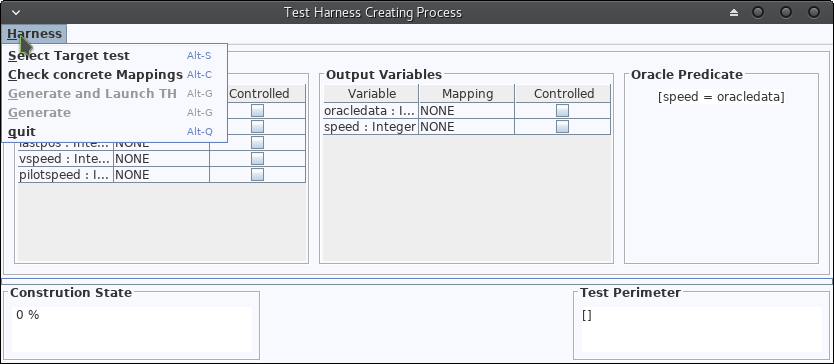
\includegraphics[scale=0.45]{images/bugquitter.png}
        \end{center}
    \end{figure} 
    
    \subsection*{Nom de véhicule bloquant}
    
    Lorsqu'on utilise \textit{Generate TH M2Alma}, si on sélectionne \textit{Select Target Test} dans le menu \textit{TestHarness Creating Process} et qu'on sélectionne SimpleVehicle avec comme seul paramètre computespeed et qu'on cherche à assigner une valeur au String vname puis qu'on annule sans valider le nom du Vehicle, il devient impossible d'assigner un String vname. La fenêtre ne réapparaît plus et le boutont devient inutilisable, nécessitant un redémarrage d'Eclipse pour pouvoir à nouveau travailler avec.


  %\clearpage
  %conclusion
  \chapter*{Conclusion}
\label{chap:conclusion}

Cette découverte de la recherche à travers un cas concret encadré nous a permis de mieux appréhender à quoi correspond le travail d'un chercheur, et de voir au travers des différentes étapes de réflexion comment ça se passe.

Nous avons mis un certain temps à réellement saisir le travail demandé car nous étions partis dans l'optique qu'on nous présente un problème et que nous devions trouver une solution qui fonctionne forcément, alors que le but de la recherche est d'émettre des hypothèses, de faire des tests pour étudier cette hypothèse et sa validité, d'en analyser les résultats et de recommencer avec une nouvelle hypothèse et donc de nouveaux tests.

Ce travail nous a sensibilisé à l'importance de la documentation de la recherche, pas juste au travers des articles et rapports à écrire en conclusion des recherches, mais surtout tout au long du processus pour garder une trace des différentes pistes suivies et pouvoir plus facilement communiquer sur le travail effectué.


  
  \bibliographystyle{unsrt}
  \bibliography{source}
  
  \section*{Annexes}

\begin{figure}
    \begin{center}
        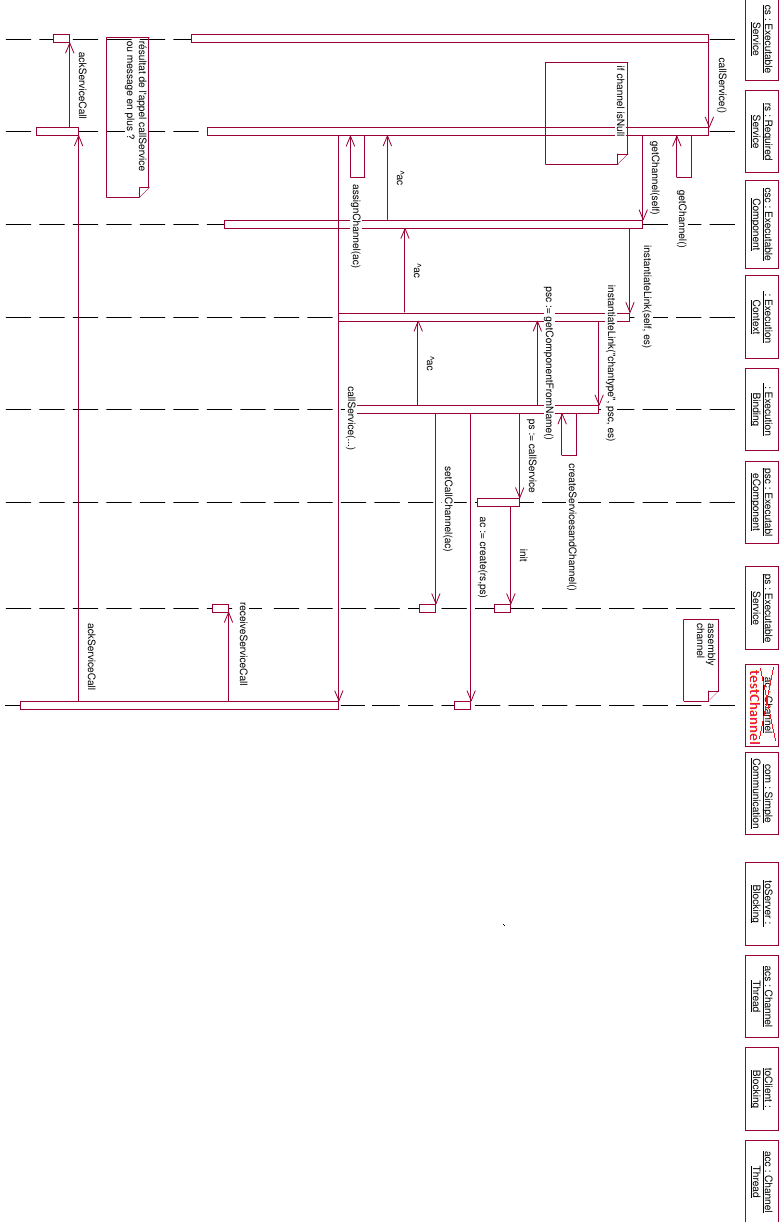
\includegraphics[scale=0.65]{images/seq.png}
        \label{annexe:callServiceSeqMock}
        \caption{Diagramme de séquence de callService avec l'utilisation du TestChannel en mock}
    \end{center}
\end{figure} 

\begin{figure}
    \begin{center}
        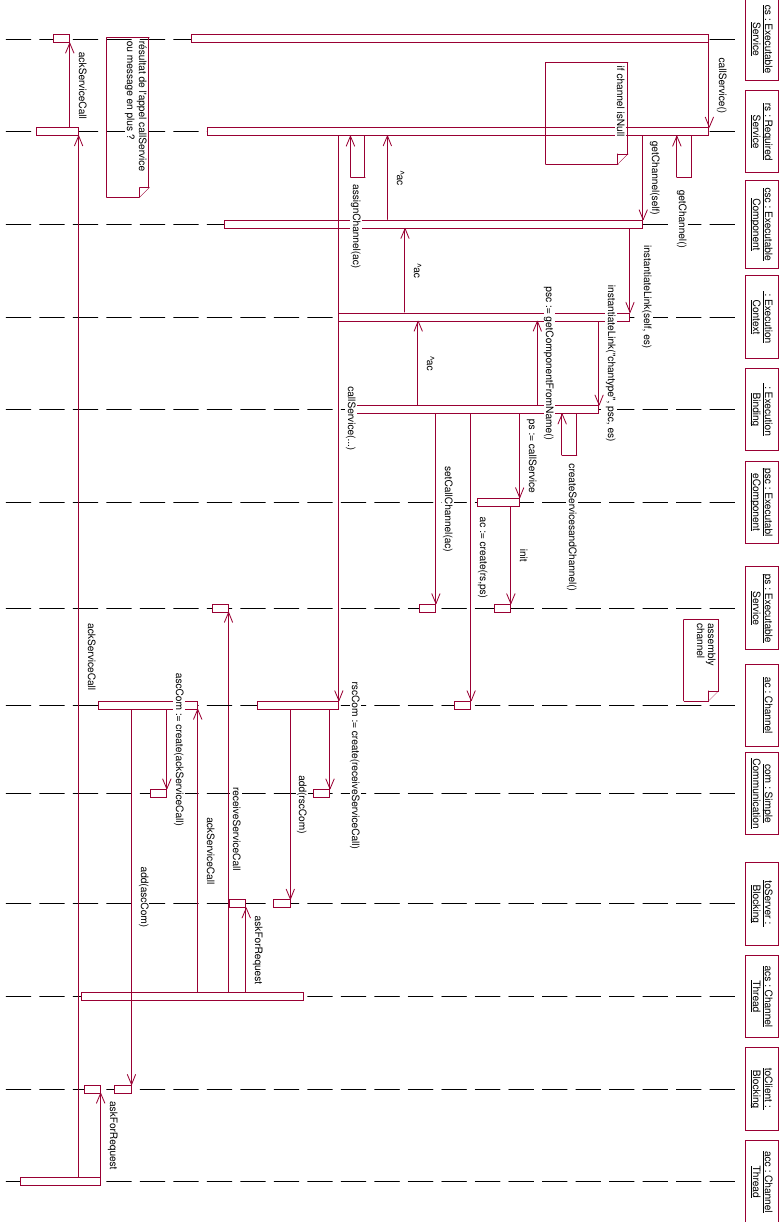
\includegraphics[scale=0.65]{images/seq1.png}
        \label{annexe:callServiceSeq}
        \caption{Diagramme de séquence de callService}
    \end{center}
\end{figure} 



%\addcontentsline{toc}{chapter}{Références}
%\bibliography{sample}
\end{document}

